\documentclass[12pt,notitlepage,twoside]{book}
\usepackage{graphicx}
\usepackage{mathptm}
\usepackage{times}
\usepackage{makeidx}
\usepackage{url}
\usepackage{supertabular}
\usepackage{MyTitlepage}
\usepackage{MyBibIndex}
\pagestyle{headings}
\makeindex
\emergencystretch=50pt
\begin{document}
\newcommand{\thesystem}{{\em Role Playing Database System}}
\newcommand{\bold}[1]{{\bf #1}}
\newcommand{\italic}[1]{{\it #1}}
\newcommand{\RPGSubTitle}{User Manual}
%* 
%* ------------------------------------------------------------------
%* Role Playing Database 2.0 by Deepwoods Software
%* ------------------------------------------------------------------
%* titlepage.tex - Generic Title Page for RPG V2.0
%* Created by Robert Heller on Sun Jul 13 18:21:56 1997
%* ------------------------------------------------------------------
%* Modification History: 
%* $Log: titlepage.tex,v $
%* Revision 1.6  2000/09/17 14:07:48  heller
%* Add cover graphic
%*
%* Revision 1.5  2000/09/17 01:13:13  heller
%* Update Copyrights
%*
%* Revision 1.4  1999/07/13 22:56:56  heller
%* Id keyword.
%* ,
%*
%* Revision 1.3  1999/05/17 23:19:20  heller
%* Update title page: copyright, web site URL.
%*
%* Revision 1.2  1998/12/26 21:59:34  heller
%* Update for RPG.
%*
%* Revision 1.1  1998/12/26 21:50:09  heller
%* Initial revision
%*
%* Revision 2.5  1998/05/17 22:07:44  heller
%* Update website info to fit better.
%*
%* Revision 2.4  1998/05/17 21:10:46  heller
%* Add website to title page.
%*
%* Revision 2.3  1998/02/08 19:15:56  heller
%* Update the copyright year
%*
%* Revision 2.2  1997/07/20 21:13:11  heller
%* Fun with \ref
%*
%* Revision 2.1  1997/07/20 20:34:53  heller
%* Squigle fun...
%*
%* Revision 2.0  1997/07/15 11:23:00  heller
%* *** empty log message ***
%*
%* ------------------------------------------------------------------
%* Contents:
%* ------------------------------------------------------------------
%*  
%*     Role Playing  Database -- a program for maintaining a database
%*                               for a Role Playing Games
%*     Copyright (C) 1997-2000  Robert Heller D/B/A Deepwoods Software
%* 			51 Locke Hill Road
%* 			Wendell, MA 01379-9728
%* 
%*     This program is free software; you can redistribute it and/or modify
%*     it under the terms of the GNU General Public License as published by
%*     the Free Software Foundation; either version 2 of the License, or
%*     (at your option) any later version.
%* 
%*     This program is distributed in the hope that it will be useful,
%*     but WITHOUT ANY WARRANTY; without even the implied warranty of
%*     MERCHANTABILITY or FITNESS FOR A PARTICULAR PURPOSE.  See the
%*     GNU General Public License for more details.
%* 
%*     You should have received a copy of the GNU General Public License
%*     along with this program; if not, write to the Free Software
%*     Foundation, Inc., 675 Mass Ave, Cambridge, MA 02139, USA.
%* 
%* $Id: titlepage.tex,v 1.6 2000/09/17 14:07:48 heller Exp $  
%* 

\title{Role Playing Database \\ A Computerized Role Playing Database System \\ \RPGSubTitle}
\author{Robert Heller \\ Deepwoods Software \\ Wendell, MA, USA}
\date{\today}
\begin{titlepage}

\maketitle

\begin{centering}
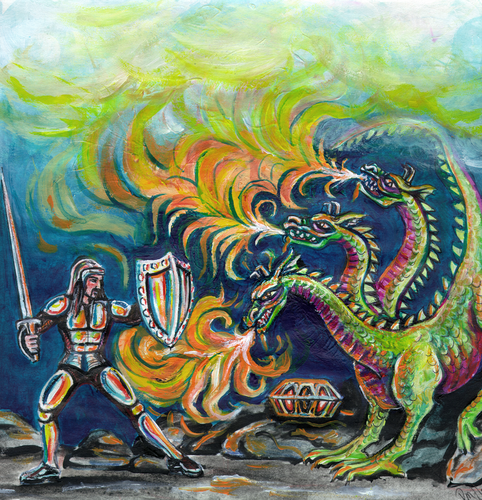
\includegraphics[height=3.5in]{Cover1.png} \\
\end{centering}

\clearpage


This documentation was prepared with \LaTeX.

This document describes version 2.1 of the Role Playing Database package.

\vspace{.25in}



{\small Copyright \copyright 1997-2000 by Robert Heller D/B/A Deepwoods
Software}

{\small Artwork Copyright \copyright 2000 By Donna Horn.}

\vspace{.25in}

All rights reserved.  Permission is granted to copy this document in
electronic form only, so long as it is with the software it
documents. 

The author, Robert Heller, may be contacted electronically (E-Mail) via
the following:

\begin{description}
\item[FidoNet] 1:321/153, Locks Hill BBS.
\item[InterNet] heller@deepsoft.com
\end{description}

Web site URL: {\tt http://www.deepsoft.com/}.

\thispagestyle{empty}
\setcounter{page}{0}
\clearpage

\end{titlepage}


\pagenumbering{roman}
\tableofcontents
\listoffigures
%%\listoftables
\cleardoublepage
%       
%* 
%* ------------------------------------------------------------------
%* Role PlayingDB V2.0 by Deepwoods Software
%* ------------------------------------------------------------------
%* Preface.tex - Preface
%* Created by Robert Heller on Wed Dec 30 11:23:20 1998
%* ------------------------------------------------------------------
%* Modification History: 
%* $Log: Preface.tex,v $
%* Revision 1.4  2000/10/09 22:29:32  heller
%* Fleshing out the text...
%*
%* Revision 1.3  2000/10/03 16:25:34  heller
%* Update Preface for commercial version.
%*
%* Revision 1.2  1999/07/14 22:17:34  heller
%* Eddy's Edits.
%*
%* Revision 1.1  1999/01/02 02:10:10  heller
%* Initial revision
%*
%* ------------------------------------------------------------------
%* Contents:
%* ------------------------------------------------------------------
%*  
%*     Role Playing DB -- A database package that creates and maintains
%* 		       a database of RPG characters, monsters, treasures,
%* 		       spells, and playing environments.
%* 
%*     Copyright (C) 1995,1998,1999  Robert Heller D/B/A Deepwoods Software
%* 			51 Locke Hill Road
%* 			Wendell, MA 01379-9728
%* 
%*     This program is free software; you can redistribute it and/or modify
%*     it under the terms of the GNU General Public License as published by
%*     the Free Software Foundation; either version 2 of the License, or
%*     (at your option) any later version.
%* 
%*     This program is distributed in the hope that it will be useful,
%*     but WITHOUT ANY WARRANTY; without even the implied warranty of
%*     MERCHANTABILITY or FITNESS FOR A PARTICULAR PURPOSE.  See the
%*     GNU General Public License for more details.
%* 
%*     You should have received a copy of the GNU General Public License
%*     along with this program; if not, write to the Free Software
%*     Foundation, Inc., 675 Mass Ave, Cambridge, MA 02139, USA.
%* 
%*  
%* 

\chapter*{Preface}
\markboth{PREFACE}{PREFACE}%
\typeout{$Id$}
\addcontentsline{toc}{chapter}{Preface}

RPGs\footnote{RPG: Role Playing Game, a game where the players take on
the roles of persons who might have lived (or may yet live) in a
different time and place.  See \cite{Gygax78,Gygax79}.} are a popular
pastime among many people these days.  Maybe they are a form of escape
from the rather mundane lives many people live, at least during the
workday.  An RPG allows the players to escape into a world where some
things are simpler, and some things more complex, in interesting
ways.

I have played AD\&D a few times and was dismayed at the amount of paperwork needed to keep track of everything.  Being a computer person, it
seemed to me that most of this paperwork could be replaced by a
computer and the information managed by a clever database system.  Given
that now there are high-powered laptop computers business people use
to keep track of and manage large corporations, it should be possible to
manage the odd imaginary universe on such a machine.  So I wrote
the \thesystem\ to manage all of the information that goes with an RPG.

The \thesystem\ maintains a database describing an RPG ``universe''.  
This ``universe'' contains a group of ``characters'', some player and
some non-player, a collection of ``monsters'', and one or more
``places'' (dungeons usually) where the ``monsters'' reside, generally
guarding some treasure.  The \thesystem\ helps game masters and players
keep track of the various things in the make-believe universe in
which the RPG takes place.

If you have {\em any} comments about this package, please let me know.
My electronic mail addresses are listed on the back side of the title
page.  I would be very interested in any comments users of the
\thesystem\ package might have.

\vspace{.25in}
\noindent
Robert Heller \\
Deepwoods Software \\
Wendell, MA, USA \\
January 1999

\section*{Addendum to the V2.1 manual}
\markboth{Preface}{Addendum to the V2.1 manual}%
\addcontentsline{toc}{section}{Addendum to the V2.1 manual}

After to talking to various people, I have made a number of upgrades to
the \thesystem, mostly colorful graphics.  I have also written in more
details into this user manual.

\section*{Addendum to the V3.0 manual}
\markboth{Preface}{Addendum to the V3.0 manual}%
\addcontentsline{toc}{section}{Addendum to the V3.0 manual}

This is a complete rewrite of the system.  Character, monster, spell, treasure,
trick/trap, and dressing ``sheets'' can be customized using a template
editor.  This allows the system to be used with any table-top RPG
system.  The data files are all ``bundled'' up as Zip archives
containing an XML file with the sheet information, plus any associated
media (graphics files or documents).  Template files are also Zip
archives containing an XML files that describe the various sheets.  Each
of these files is self-contained and can be carried from computer to
computer on the media of your choice (eg CD/DVD-Rs, thumb drives, flash
cards, etc.).  Map files are also Zip archives containing an XML files
along with any associated media (graphics files or documents).

\vspace{.25in}
\noindent
Robert Heller \\
Deepwoods Software \\
Wendell, MA, USA \\
October 2000

%
\cleardoublepage
\pagenumbering{arabic}
%
%* 
%* ------------------------------------------------------------------
%* Role PlayingDB V2.0 by Deepwoods Software
%* ------------------------------------------------------------------
%* IntroUserManual.tex - User Manual Introduction
%* Created by Robert Heller on Wed Dec 30 11:22:15 1998
%* ------------------------------------------------------------------
%* Modification History: 
%* $Log: IntroUserManual.tex,v $
%* Revision 1.4  2000/10/09 22:29:32  heller
%* Fleshing out the text...
%*
%* Revision 1.3  1999/07/14 23:23:46  heller
%* Small last minute update.
%*
%* Revision 1.2  1999/07/14 22:17:34  heller
%* Eddy's Edits.
%*
%* Revision 1.1  1999/01/02 02:11:05  heller
%* Initial revision
%*
%* ------------------------------------------------------------------
%* Contents:
%* ------------------------------------------------------------------
%*  
%*     Role Playing DB -- A database package that creates and maintains
%* 		       a database of RPG characters, monsters, treasures,
%* 		       spells, and playing environments.
%* 
%*     Copyright (C) 1995,1998  Robert Heller D/B/A Deepwoods Software
%* 			51 Locke Hill Road
%* 			Wendell, MA 01379-9728
%* 
%*     This program is free software; you can redistribute it and/or modify
%*     it under the terms of the GNU General Public License as published by
%*     the Free Software Foundation; either version 2 of the License, or
%*     (at your option) any later version.
%* 
%*     This program is distributed in the hope that it will be useful,
%*     but WITHOUT ANY WARRANTY; without even the implied warranty of
%*     MERCHANTABILITY or FITNESS FOR A PARTICULAR PURPOSE.  See the
%*     GNU General Public License for more details.
%* 
%*     You should have received a copy of the GNU General Public License
%*     along with this program; if not, write to the Free Software
%*     Foundation, Inc., 675 Mass Ave, Cambridge, MA 02139, USA.
%* 
%*  
%* 

\chapter{Introduction}
\label{Intro}
\typeout{$Id$}
\section{What Is the \thesystem?}

The \thesystem\ is a specialized database system with a GUI front end
designed to aid people who play RPGs.  Both the players and the masters
can find uses for this package, to manage the information that
describes the players' characters and the game environment and its
contents.

The system consists of a collection of Tcl/Tk (\cite{Ousterhout94})
script files that implement a GUI-based program that maintains data
files that describe the various elements used in table-top
role playing games. The main elements consist of characters, both those
played by the players and those ``played'' by the game master.
Additional elements consist of monsters, spells, treasure, tricks /
traps, random additional objects, plus the maps and descriptive
information of the game playing locale.  See \cite{HellerRPGTcl09} for a
detailed description of these script files.

\section{How this Manual Is Organized}

Chapter~\ref{Reference} is a basic reference manual, describing the
eight main toplevel GUI windows:

\begin{enumerate}

\item The {\em Main} window.  This is the main window and it is
described in detail in Section~\ref{Main}.  The main window is the main
start up screen and contains the means to navigate to other parts of the
program.

\item The {\em Sheet Template Editor} window.  This window is used to
edit the structure and contents of a ``sheet'' (Character, Monster,
Spell, Treasure, Trick / Trap, or Dressing).  This window is described
in detail in Section~\ref{Template}.

\item The {\em Character Editing} window.  This window is used to create
and edit Character Object data files and it is described in detail in
Section~\ref{Character}. 

\item The {\em Monster Editing} window.  This window is used to create
and edit Monster Object data files and it is described in detail in
Section~\ref{Monster}. 

\item The {\em Spell Editing} window.  This window is used to create
and edit Spell Object data files and it is described in detail in
Section~\ref{Spell}. 

\item The {\em Treasure Editing} window.  This window is used to create
and edit Treasure Object data files and it is described in detail in
Section~\ref{Treasure}. 

\item The {\em Trick / Trap Editing} window.  This window is used to create
and edit Trick or Trap Object data files and it is described in detail in
Section~\ref{TrickTrap}. 

\item The {\em Dressing Editing} window.  This window is used to create
and edit Dressing Object data files and it is described in detail in
Section~\ref{Dressing}. 

\item The {\em Map Editing} window.  This window is used to create
and edit Map Object data files and it is described in detail in
Section~\ref{Map}. 

\end{enumerate}


Chapter~\ref{Tutorial} is a step-by-step tutorial that takes the reader
through the process of creating a game system template, informational
sheets for characters, monsters, etc. and the creation of a map of the
game playing realm.

\chapter{Reference}
\label{Reference}
\typeout{$Id$}

\section{Main Window}
\label{Main}

\begin{figure}[hbpt] \begin{centering}
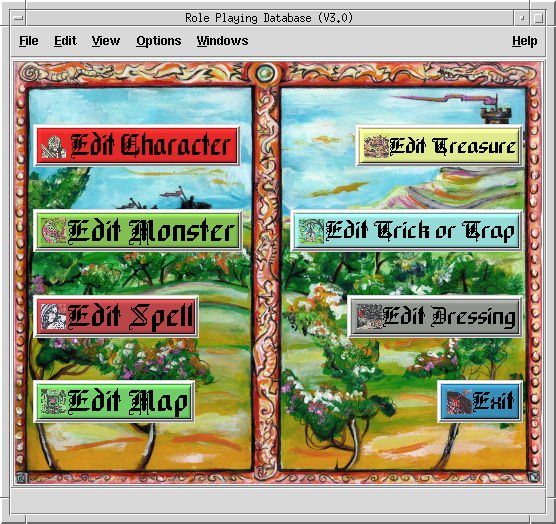
\includegraphics[width=5in]{MainWindow.png} \caption{The main window of
the Role Playing Database} \label{fig:main} \end{centering}
\end{figure} The main window, shown in Figure~\ref{fig:main}, contains
buttons for the seven game informational editors: Character, Monster,
Spell, Treasure, Trick / Trap, Map, and Dressing.  See
Section~\ref{SheetEditor} for a documentation on the Character,
Monster, Spell, Treasure, Trick / Trap, Dressing editor windows and
Section~\ref{Map} for documentation the Map editor window. An eighth
button selects for program exit. In addition to the eight buttons,
there are drop down menus on a menu bar.  The same menu bar is used on
all of the major top level screens.  The File menu has the standard
New, Open, Save, Save As, Print, Close, and Exit menu items, all of
which have the expected meanings and functionality.  The New and Open
menu items on the File menu use cascading menus to select the sort of
thing to create or open.  The Options menu contains menu items to
create/edit (see Section~\ref{sect:configuration}), read, and write the
program's main configuration file, plus a menu item to edit template
files, which opens the ``Sheet Template Editor'' window (See
Section~\ref{Template}), which is used to create and maintain the sheet
editor windows.  The Windows menu contains menu items to select one of
the existing top level windows. The Help menu provides access to the
on line help system (see Chapter~\ref{Help} for complete information
about using the on-line help).

\section{Configuration Editor}
\label{sect:configuration}

\begin{figure}[hbpt]
\begin{centering}
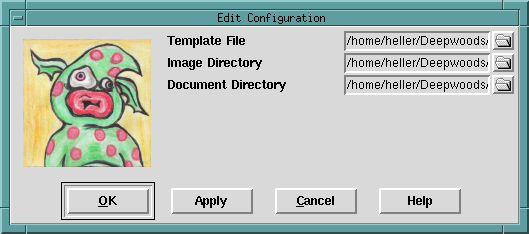
\includegraphics[width=5in]{ConfigurationEditor.png}
\caption{The Configuration Editor Window}
\label{fig:confedit}
\end{centering}
\end{figure}
In Figure~\ref{fig:confedit} is shown the Configuration Editor Window. 
There are three configuration options: the template file to use when
creating new informational sheets, the initial directory to look in for
images for graphic elements, and the initial directory to look in for
external documents.  The configuration file is located in the current
user's home directory in a file named \verb=.roleplayingdb3= under
UNIX/Linux and MacOSX and \verb=roleplayingdb3.rc= under MS-Windows. 
This file is a plain text file containing key, value pairs.  Do not edit
this file by hand though.  Be sure to use the Configuration Editor. 
This makes sure that the file is properly formatted to be read in at
program start time.

\section{Sheet Template Editor Window}
\label{Template}

\begin{figure}[hbpt]
\begin{centering}
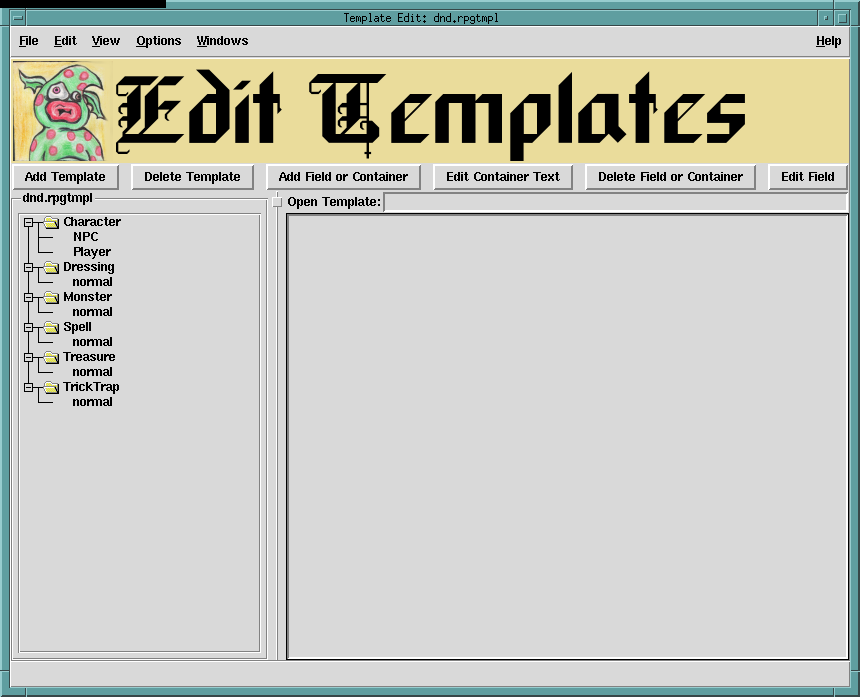
\includegraphics[width=5in]{TemplateEditor1.png}
\caption{The initial Template Editor Window}
\label{fig:tmped1}
\end{centering}
\end{figure}
\begin{figure}[hbpt]
\begin{centering}
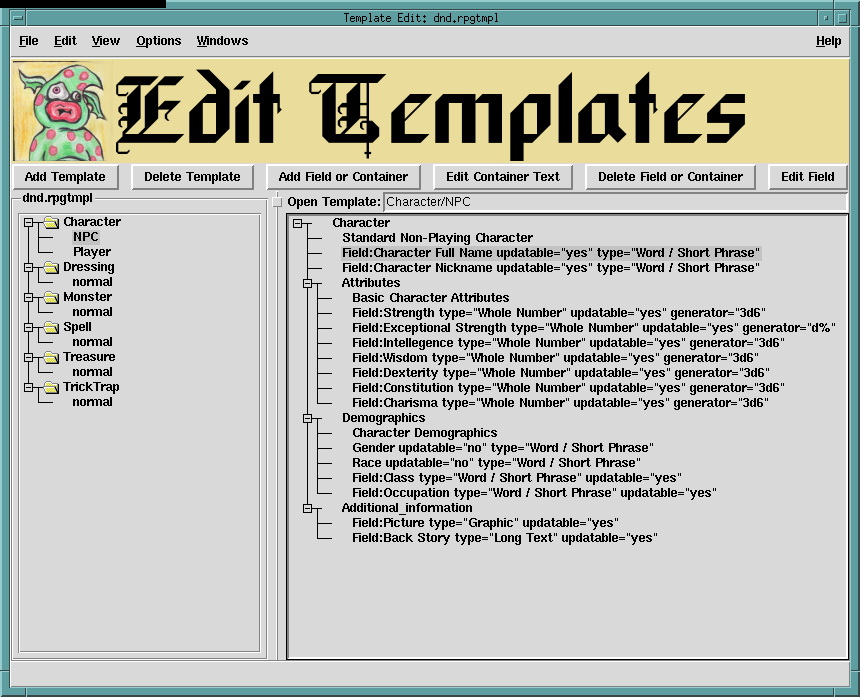
\includegraphics[width=5in]{TemplateEditor2.png}
\caption{The Template Editor Window after loading a template}
\label{fig:tmped2}
\end{centering}
\end{figure}
To allow for differences in game systems, game data elements are
defined with the use of templates.  These templates define what
information is recorded for each game element for a given game system. 
These templates are created and maintained with the template editor. 
The template editor in invoked from the Options menu.  The editor is
shown in Figures~\ref{fig:tmped1} and \ref{fig:tmped2}.  A sheet
contains a top level container which in turn contains zero or more fields
or containers.  Containers can contains zero or more fields or
containers.  Fields and containers have names. Fields also have a type,
possibly a generator (dice combination), and a flag that indicates whether the
field value can be updated.  There are five defined field types:

\index{Field types|(}
\begin{enumerate}
\item \verb=Whole Number=--This is a numerically valued field. It is either
an arbitrary (usually fixed) value or the result of a dice throw.
\item \verb=Word / Short Phrase=--This either a single word or a short
(one line at most) phrase, generally describing a textual attribute,
such as a name or some sort of descriptive condition or status.
\item \verb=Long Text=--This is a multi-line, but short (1-2 paragraph)
text value.
\item \verb=Graphic=--This is a picture file.  Most standard graphics
formats are supported, including GIF, PNG, JPEG, BMP, TIFF, TGA,
PostScript, and Sun Raster.  The graphic file will be displayed in the
sheet editor window.
\item \verb=Document=--This a document file.  Any sort of external file
is supported.  The external file will be copied into the sheet file. 
The sheet editor will not attempt to display or otherwise process the
file, but since the file will be ``carried'' along with the sheet file,
it will be available and extractable as needed.
\end{enumerate}
\index{Field types|)}

The generator attribute is only used for numerically valued fields and
the updatable attribute can only be set to no for the word / short
phrase and numerically valued fields.

The templates are used for Character, Monster, Spell, Treasure, Trick /
Trap, and Dressing sheet editors.  The Map editor uses a set of hard-coded
templates. These templates define the fields, their attributes, and
grouping / organizational structure.  Containers have a text attribute
that is used as a section heading for the group of fields contained in
the container. The included template file, \verb=dnd.rpgtmpl=, defines
informational sheets suitable for \textit{Advanced Dungeons and
Dragons}, but template files for other game systems can be created.

A template file is a Zip archive file containing directories for each
class of sheet: Character, Monster, Spell, Treasure, Trick / Trap, and
Dressing.  These directories in turn contain the template XML files,
which define the structure of the sheets.  It is possible to have
multiple templates for any given class.  It is also possible to have no
templates for a given class.  Not all game systems have all classes of
these things and others might have several sub-classes, sometimes with
very different attributes.

\section{Sheet Editor Windows}
\label{SheetEditor}

\begin{figure}[hbpt]
\begin{centering}
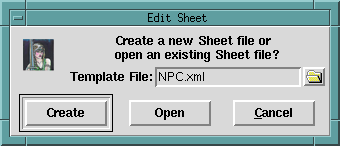
\includegraphics{CreateOrOpenChar.png}
\caption{The Open or Create Character dialog box}
\label{fig:opencreatechar}
\end{centering}
\end{figure}
\begin{figure}[hbpt] 
\begin{centering}
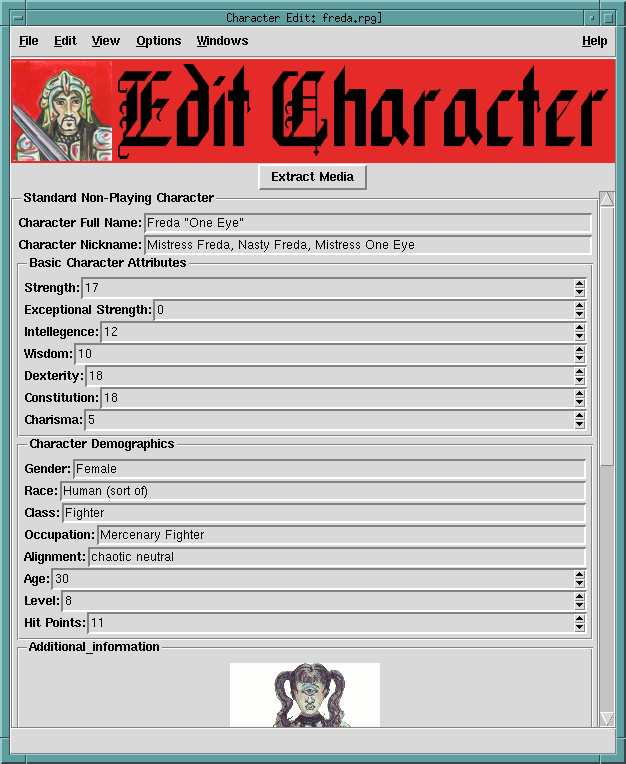
\includegraphics[width=5in]{CharacterEditor.png} 
\caption{The Character Editor window of the Role Playing Database} 
\label{fig:char}
\end{centering} 
\end{figure} 
The Sheet Editor Window, which includes the Character Editor, shown in
Figure~\ref{fig:char}, is used to edit characters, both playing and
non-playing characters, monsters, spells, treasure, tricks / traps, and
dressing items.  It uses one of the sheet templates defined in the
current template file (see Section~\ref{sect:configuration}).  When one
of the sheet editor buttons on the main window are clicked on, a small
dialog box is displayed (shown in Figure~\ref{fig:opencreatechar}),
asking if you want create a new sheet file, using a selected template
or open an existing sheet file. The Monster, Spell, Treasure,  Trick /
Trap, and Dressing Editor Windows are the same as the Character Editor,
but use different templates.

In addition to the fields created from the sheet template, there is also
a tool bar button, labeled ``Extract Media''.  This button allows for the
extraction of embedded media files contained within the sheet file. 
This allows for the use of external editors or viewers with these files.

A sheet file is a Zip archive containing two directories, xml and media.
The xml contains a file named sheet.xml, which is an XML file containing
the sheet information.  The media directory contains any media files
associated with the sheet--this could be pictures or other documents.

\section{Map Editing Windows}
\label{Map}

Map objects are three dimensional, consisting of one or more levels,
above, below, or at ground level.  Each level consists of spaces
(squares or hexagons) arranged on a two dimensional grid.  Each level
is at a depth, where a depth of 0 is ground level, negative depths are
below ground, and positive depths are above ground.  Spaces have an X
and Y coordinate, which are whole numbers ranging between -1000 and
1000, with 0 being the center of the level and -1000 being the extreme
left or western edge (X) and extreme top or northern edge (Y) and 1000
being the extreme right or eastern edge (X) and extreme bottom or
southern edge (Y). Creating or editing a map is a hierarchical process. 
You select the level to create or edit from the main map window
(Figure~\ref{fig:MapEditor}) and you select the space to create or edit
from the level editor window (Figure~\ref{fig:LevelEditor}) for the
level the space is on.  The whole map, with all of its levels and
spaces are stored in a single file, for easy transport and exchange.  It
is possible to have a ``sparse'' map, with levels and/or spaces
omitted.  These might be levels or spaces that have not been
constructed (yet) or are otherwise inaccessible.  With suitable
technology or magic (eg a teleport device or spell) it is possible to
get to non-adjacent spaces or levels.  No attempt it made it enforce
connectivity to adjacent spaces or levels!

There are three map editing windows:
\begin{enumerate}
\item The main map editor, shown in Figure~\ref{fig:MapEditor}, contains
information about the overall map, including the name of the map, the
name of the campaign, and the name of the game master.  This window is
described in Section~\ref{sect:mainmap}.
\item The level editor, shown in Figure~\ref{fig:LevelEditor}, contains
information about a selected level. This window is
described in Section~\ref{sect:leveledit}.
\item The space editor, shown in Figure~\ref{fig:SpaceEditor}, contains
information about a space. This window is
described in Section~\ref{sect:spaceedit}.
\end{enumerate}

\subsection{Main map editing window}
\label{sect:mainmap}

\begin{figure}[hbpt] 
\begin{centering}
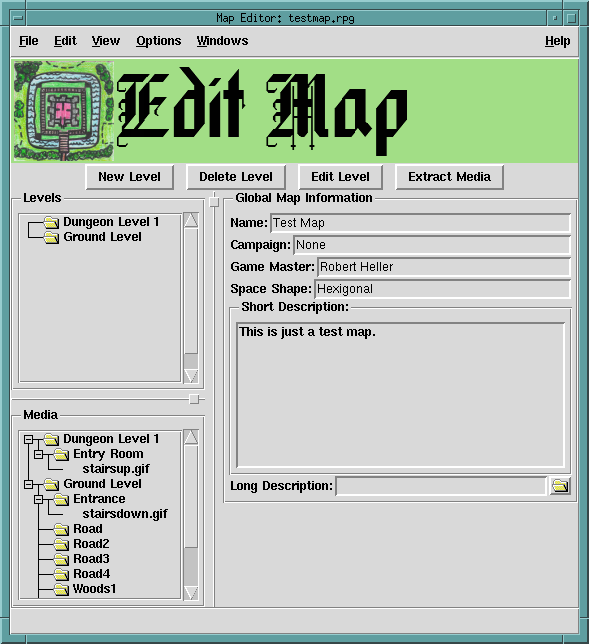
\includegraphics[width=5in]{MapEditor.png}
\caption{Main map editor window}
\label{fig:MapEditor}
\end{centering}
\end{figure}
The main map editor (Figure~\ref{fig:MapEditor}) contains information
about the overall map.  This information includes name of the map, the
name of the campaign, and the name of the game master.  There is space
for a brief description of the map and it is possible to include a
larger document providing a detailed writeup about the map or game
campaign.  Also on this window is a list of levels and a directory tree
of included media.  There is a tool bar with 4 buttons:

\begin{enumerate}
\item New Level--this button creates a new level.
\item Delete Level--this button deletes a selected level.
\item Edit Level--this button edits a selected level.
\item Extract Media--this button extracts a selected media file, making
it available for an external program to view or otherwise process.
\end{enumerate}

\subsection{Level editing window}
\label{sect:leveledit}

\begin{figure}[hbpt] 
\begin{centering}
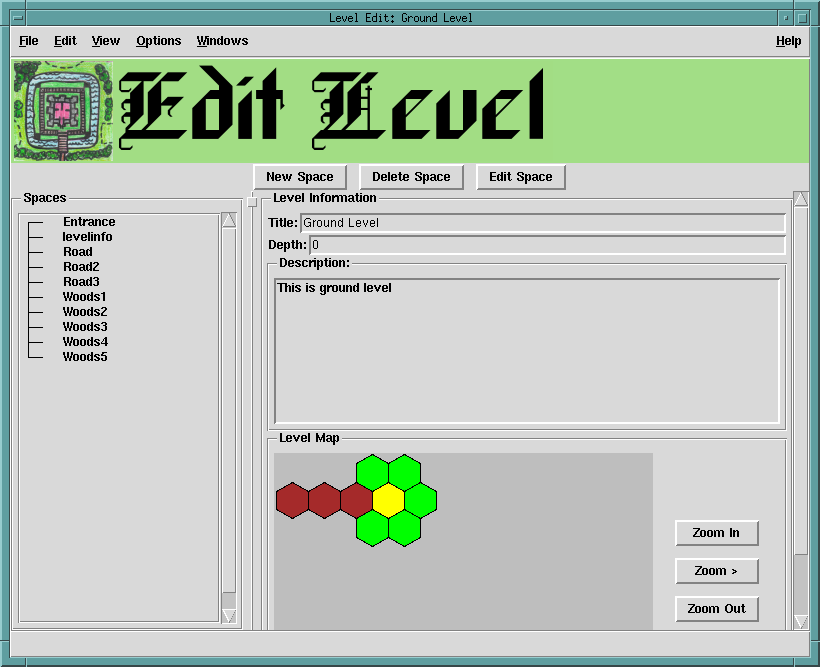
\includegraphics[width=5in]{LevelEditor.png}
\caption{Level editor window}
\label{fig:LevelEditor}
\end{centering}
\end{figure}
The level editor (Figure~\ref{fig:LevelEditor}) contains information
about a selected level.  This information includes the title of the
level and its depth (positive depths are above ground, negative depths are
below ground and a depth of zero is at ground level).  Also included is
a space for a brief description of the level and a map of the level as
well as a list of spaces.

There is a tool bar with three buttons:
\begin{enumerate}
\item New Space--This button creates a new space.
\item Delete Space--This button deletes an existing space.
\item Edit Space--This button edits an existing space.
\end{enumerate}

\subsection{Space editing window}
\label{sect:spaceedit}

\begin{figure}[hbpt] 
\begin{centering}
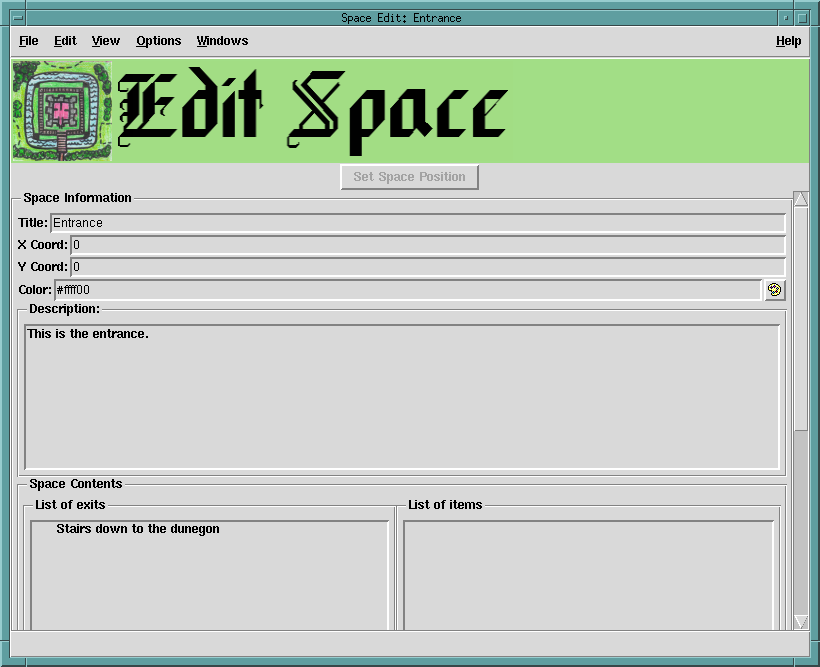
\includegraphics[width=5in]{SpaceEditor.png}
\caption{Space editor window}
\label{fig:SpaceEditor}
\end{centering}
\end{figure}
The space editor (Figure~\ref{fig:SpaceEditor}) contains information
about a selected space.  This information includes the title of the
space, its X and Y coordinates, its color and a short description. 
There is also a pair of lists, one of exits from this space to another
space and a list of other items in the space (such as treasure,
monsters, tricks, traps, and any other odds and ends).  There is also a
map of the space, showing the location of every listed exit or item in
the space.

Below the item and exit lists are triplets of buttons: adding,
deleting, and editing an item or exit.  The main difference between an
item and an exit is that exits have a ``pointer'' to a space and level.
Otherwise, both have a name, a short description, a location within
the space, a graphic, and a sheet file.  The location is an X,Y value,
where the  X and Y values range between -320 and 320, where 0,0 is the
center of the space.  This location is just a relative location within
the space and does not represent any particular distance, other than
that -320 represents the top (Y) or left (X) sides and 320 represents
the bottom (Y) or right (X) side.  The sheet file is optional (this
would make sense if the item or exit was a trick, trap, treasure,
monster, etc.).

When a space is first created, there is available a tool bar button that
can be used to position the space with the mouse.  Once the space has
been saved, its location is fixed and it cannot be moved.  The ``color'' is
arbitrary and is used to color the space on the level map and it is also
used as the space's background color on the space map in the space
editor.  This of course makes it easier to keep track of where spaces
are on the level map.  A game master can use the colors to ``code''
different spaces as having some particular property or feature, such as
coloring wooded areas green and mountainous areas brown and towns with
yellow and castles in blue for example.

\section{Printing}

All main windows have a \verb=Print...= menu item on the \verb=File=
menu. Except for the main window, this menu item allows you to print the
sheet, template, map, level, or space to a PDF file.  At present there
is no support to print directly to your printer, but there are many
programs to print a PDF file to a printer.  A PDF file can also be
shared with someone who does not have the Role Playing Database system
or a PDF file can be uploaded to a website or posted to a blog.  The
\verb=Print...= menu item will ask for the name of the file to be
created.  In the case of the Map and Level editors, you also have the
option of printing the levels (in the case of a Map editor window) or
the spaces (in the case of a Level editor window) or not.

\chapter{Tutorial}
\label{Tutorial}
\typeout{$Id$}

\section{Creating a Template Bundle}

To create information sheets for your game elements, you will need to
create templates\footnote{A pre-built template bundle for
\textit{Advanced Dungeond and Dragons}, dnd.rpgtmpl, is included, so if
you play using the \textit{Advanced Dungeond and Dragons} system, you
are all set to go.}.

\begin{figure}[hbpt] 
\begin{centering}
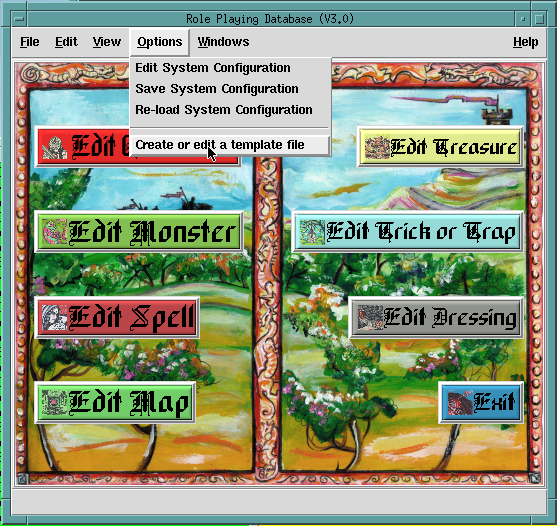
\includegraphics[width=5in]{OptionMenu.png} 
\caption{Selecting ``Create or edit a template file''} 
\label{fig:createoredittemplatemenu} 
\end{centering}
\end{figure} 
\begin{figure}[hbpt] 
\begin{centering}
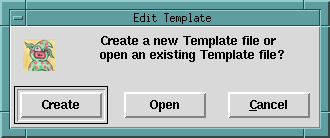
\includegraphics{CreateOrEditTemplateDialog.png} 
\caption{The Create Or Edit Template Dialog}
\label{fig:createoredittemplate} 
\end{centering}
\end{figure} 
\begin{figure}[hbpt]
\begin{centering}
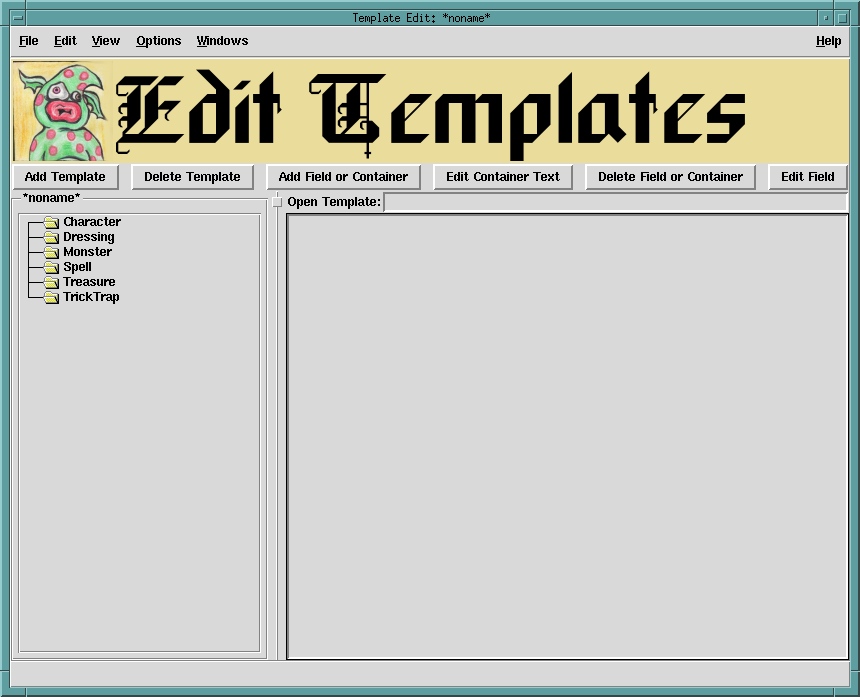
\includegraphics[width=5in]{EmptyTemplateEditor.png}
\caption{Empty Template Editor Window}
\label{fig:emptytemplate}
\end{centering}
\end{figure}
\begin{figure}[hbpt]
\begin{centering}
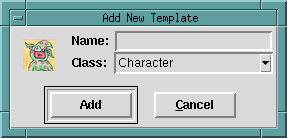
\includegraphics{AddNewTemplate.png}
\caption{Add New Template Dialog Box}
\label{fig:addnewtemplate}
\end{centering}
\end{figure}
\begin{figure}[hbpt]
\begin{centering}
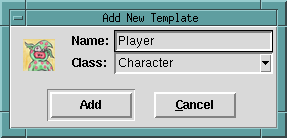
\includegraphics{AddNewTemplatePlayer.png}
\caption{Add New Template Dialog Box, with ``Player'' filled in}
\label{fig:addnewtemplateplayer}
\end{centering}
\end{figure}
\begin{figure}[hbpt]
\begin{centering}
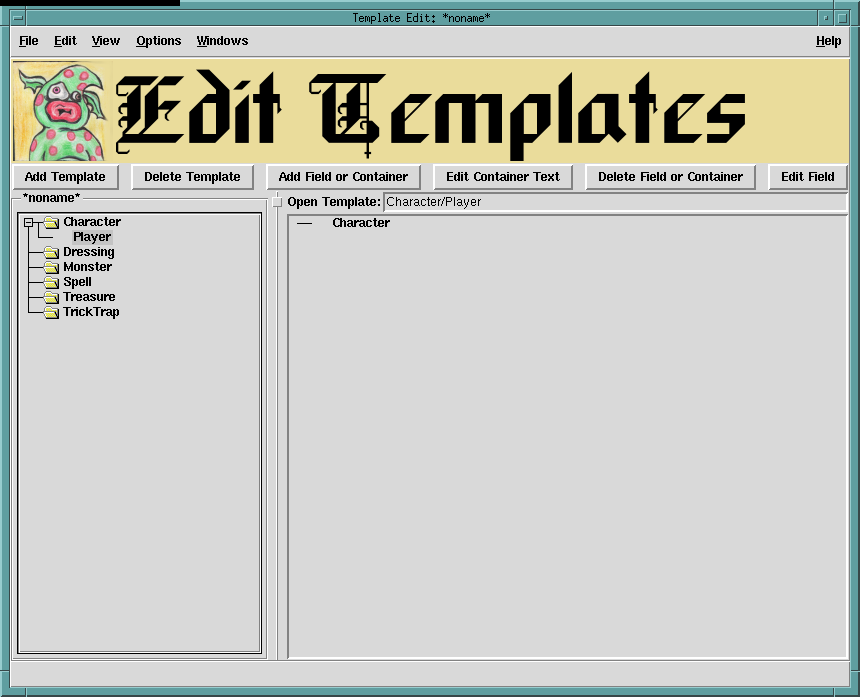
\includegraphics[width=5in]{PlayerTemplateEditor.png}
\caption{Template Editor, with empty ``Player'' template}
\label{fig:emptyplayertemplateeditor}
\end{centering}
\end{figure}
To create a template bundle, select ``Create or edit a template file''
from the Options menu, as shown in
Figure~\ref{fig:createoredittemplatemenu}.  This will display the dialog box
shown in Figure~\ref{fig:createoredittemplate}.  Select ``Create''.  An
empty template editor window, as shown in Figure~\ref{fig:emptytemplate}
will be opened up.  You can now start to create templates for your game
system.  We will create a simple Character class template.  First, click
on ``Add Template''.  This will open up the ``Add New Template'' dialog
box, as shown in Figure~\ref{fig:addnewtemplate}.  Type ``Player'' in
the name field, as shown in Figure~\ref{fig:addnewtemplateplayer}, and
click ``Add''.  This will create an entry under the ``Character'' folder
named ``Player''.  Double click on this entry now.  The template editor
will will now look like Figure~\ref{emptyplayertemplateeditor}.

\subsection{Adding heading text to a container}

\begin{figure}[hbpt]
\begin{centering}
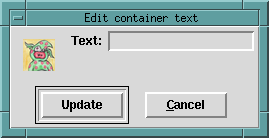
\includegraphics{EmptyEditContainerText.png}
\caption{Empty ``Edit Container Text'' dialog box}
\label{fig:editcontainertext}
\end{centering}
\end{figure}
\begin{figure}[hbpt]
\begin{centering}
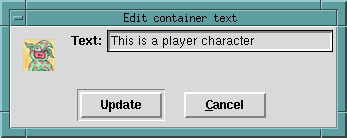
\includegraphics{EditContainerTextWithText.png}
\caption{``Edit Container Text'' dialog box with text added}
\label{fig:editcontainertextwithtext}
\end{centering}
\end{figure}
\begin{figure}[hbpt]
\begin{centering}
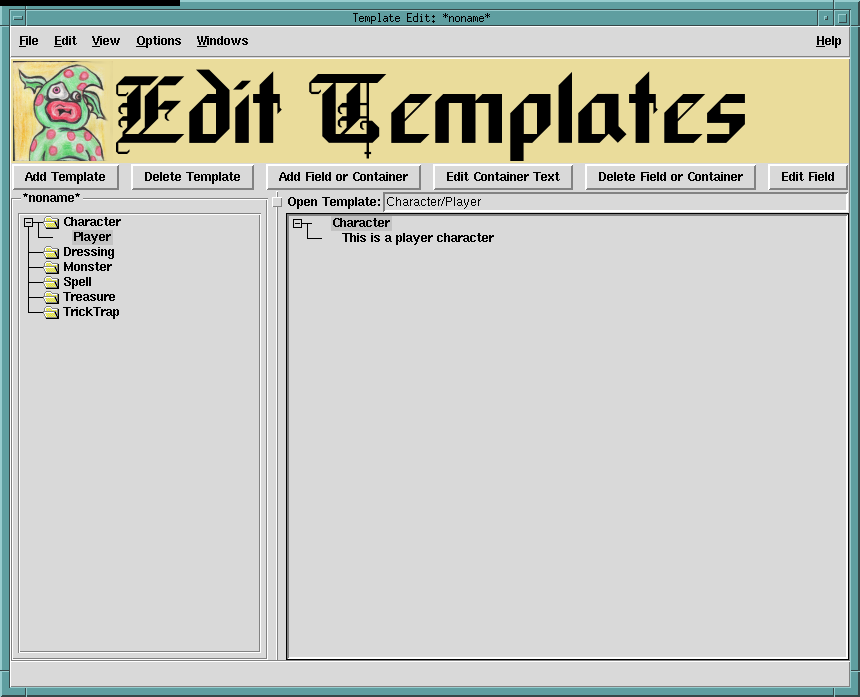
\includegraphics[width=5in]{PlayerTemplateEditorHeading.png}
\caption{Template Editor, with ``Player'' template, with a heading added}
\label{fig:playertemplateeditorwithheading}
\end{centering}
\end{figure}
At first, all that is in a sheet template is an empty toplevel
container, named for the class of sheet (Character) in this case.  The
first thing you will want to do is add a heading for this container.
Highlight the container name by clicking on it, then click the ``Edit
Continer Text'' button on the tool bar.  This will display the ``Edit
Container Text'' dialog box, as shown in
Figure~\ref{fig:editcontainertext}. Fill in the text field with ``This
is a player character''.  The dialog box will now look like
Figure~\ref{fig:editcontainertextwithtext}. Click ``Update''. The
template editor window will now look like
Figure~\ref{fig:playertemplateeditorwithheading}.

\subsection{Adding a field to a container}

\begin{figure}[hbpt]
\begin{centering}
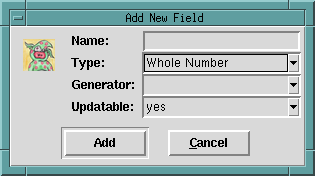
\includegraphics{AddNewFieldDialog.png}
\caption{``Add New Field'' dialog box}
\label{fig:addnewfield}
\end{centering}
\end{figure}
\begin{figure}[hbpt]
\begin{centering}
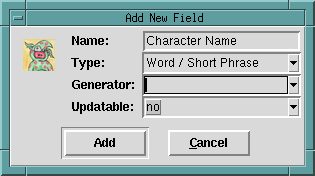
\includegraphics{AddNewFieldDialogWithField.png}
\caption{``Add New Field'' dialog box with field values filled in}
\label{fig:addnewfieldfilledin}
\end{centering}
\end{figure}
\begin{figure}[hbpt]
\begin{centering}
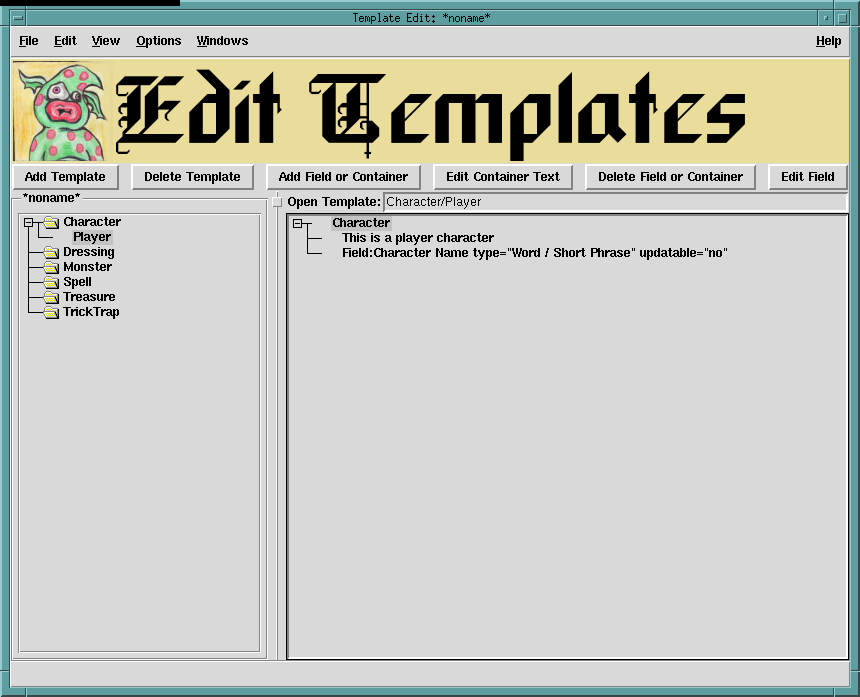
\includegraphics[width=5in]{PlayerTemplateEditorWithField.png}
\caption{Template Editor, with ``Player'' template, with a field added}
\label{fig:playertemplateeditorwithfield}
\end{centering}
\end{figure}
To add a field to the toplevel container, make sure the container name
is highlighter (click on the name to be sure), and click on the ``Add
Field or Container''.  This will display the ``Add New Field'' dialog
box, shown in Figure~\ref{fig:addnewfield}.  Fill in the ``Name'' field
with ``Character Name'', select ``Word / Short Phrase'' from the
``Type'' menu, and set ``Updatable'' to ``no''.  The dialog box should
now look like Figure~\ref{fig:addnewfieldfilledin}.  Click the ``Add''
button on the dialog box.  The template editor window should now look
like Figure~\ref{fig:playertemplateeditorwithfield}.

\subsection{Adding a container to a container}

\begin{figure}[hbpt]
\begin{centering}
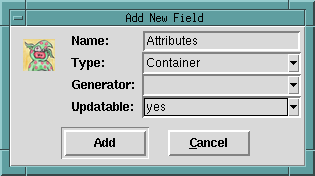
\includegraphics{AddNewFieldDialogWithContainer.png}
\caption{``Add New Field'' dialog box with container}
\label{fig:addnewcontainer}
\end{centering}
\end{figure}
\begin{figure}[hbpt]
\begin{centering}
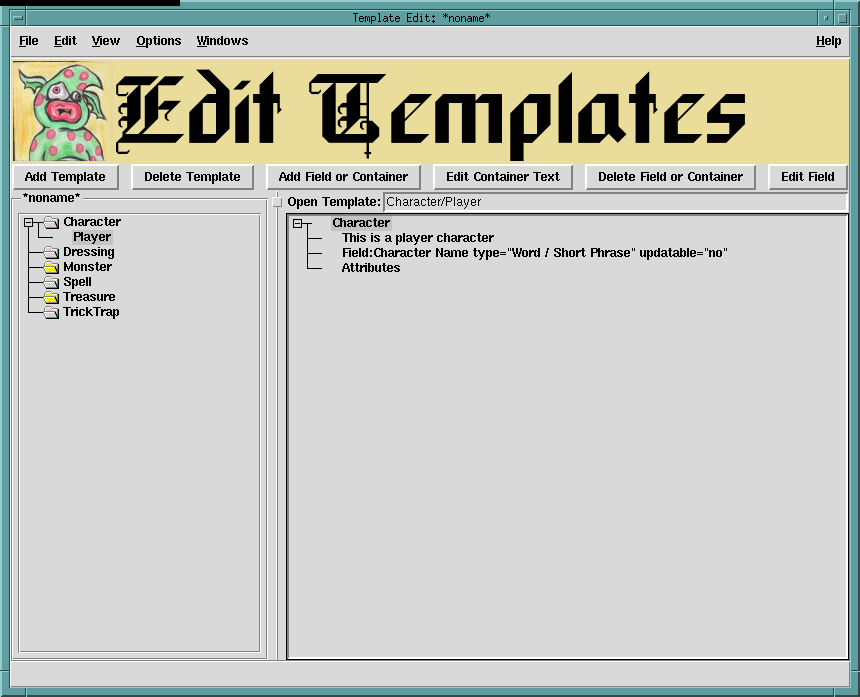
\includegraphics[width=5in]{PlayerTemplateEditorWithContainer.png}
\caption{Template Editor, with ``Player'' template, with a container added}
\label{fig:playertemplateeditorwithcontainer}
\end{centering}
\end{figure}
To add a container to the toplevel container, make sure the container name
is highlighter (click on the name to be sure), and click on the ``Add
Field or Container''.  This will display the ``Add New Field'' dialog
box, shown in Figure~\ref{fig:addnewfield}.  Fill in the ``Name'' field
with ``Attributes'', select ``Container'' from the
``Type'' menu, and set ``Updatable'' to ``yes''.  The dialog box should
now look like Figure~\ref{fig:addnewcontainer}.  Click the ``Add''
button on the dialog box.  The template editor window should now look
like Figure~\ref{fig:playertemplateeditorwithcontainer}.

\section{Creating a character sheet}

\begin{figure}[hbpt]
\begin{centering}
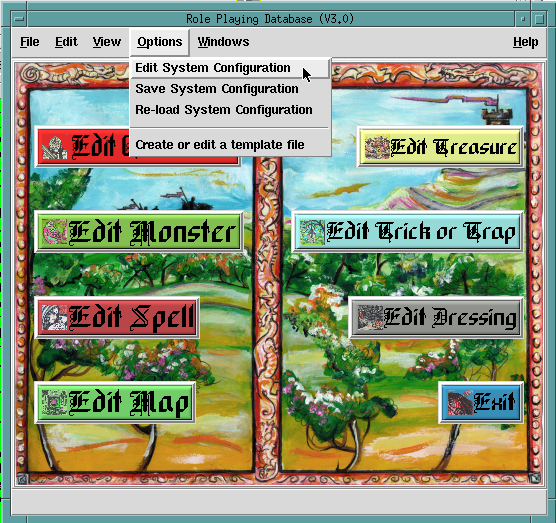
\includegraphics{OpenConfigurationEditor.png}
\caption{Selecting ``Edit System Configuration'' from the ``Options'' menu}
\label{fig:opensysconfedit}
\end{centering}
\end{figure}
To create a character sheet, we first need to be sure that there is an
available template bundle.  Go to the \verb=Options= menu and select
\verb=Edit System Configuration=, as shown in
Figure~\ref{fig:opensysconfedit}. Click on the file folder button to the
right of the ``Template File'' field and navigate to the location of the
\verb=dnd.rpgtmpl= file included with the \thesystem. Click ``Open'' on
the file select dialog and then ``OK'' on the configuration editor
window.  You might want then go to the \verb=Options= menu and select
\verb=Save System Configuration= to write out this configuration.

\begin{figure}[hbpt]  
\begin{centering}
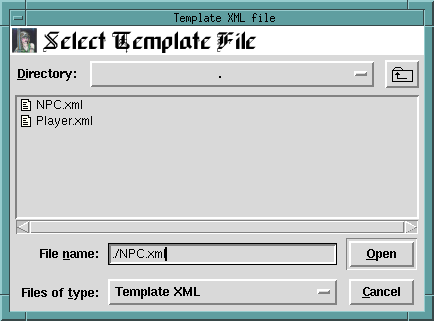
\includegraphics{SelectTemplateFile.png} 
\caption{The ``Select Template File'' dialog} 
\label{fig:selecttemplatefile} 
\end{centering}
\end{figure} 
\begin{figure}[hbpt] 
\begin{centering}
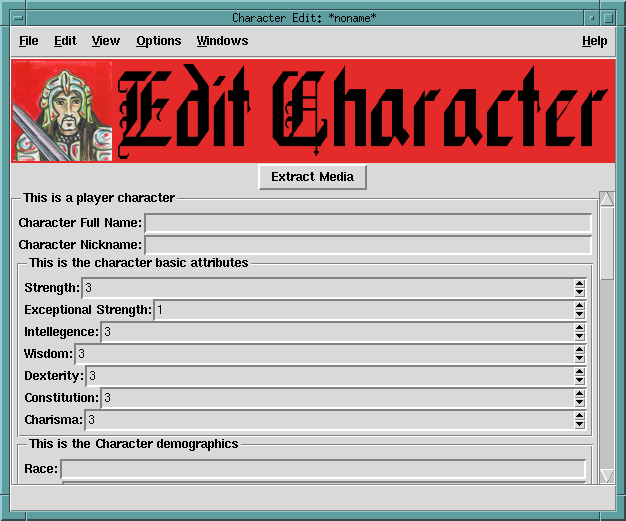
\includegraphics[width=5in]{EmptyPlayerCharacterSheet.png} 
\caption{An empty player character sheet} 
\label{fig:emptyplayercharacter}
\end{centering} 
\end{figure} 
Next, click on the \verb=Edit Character= button.  This will open the
``Open or Create Character'' dialog box, shown in
Figure~\ref{fig:opencreatechar}.  Click on the file folder button. 
This will open the ``Select Template File'' dialog, shown in
Figure~\ref{fig:selecttemplatefile}. Double click on ``Player.xml''. 
This will select the player template, rather than the default
non-player character (NPC) template.  Now click on the ``Create''
button on the ``Open or Create Character'' dialog box.  You should now
have an empty character sheet much like that shown in
Figure~\ref{fig:emptyplayercharacter}. You are now ready to create a
player character sheet!  The process is much like filling in a form.
Each piece of information is filled into a labeled space.  Numeric
values have small up and down arrows at the right end of the field and
you can either type in the numbers or use these arrows to increase or
decrease the value in the field.  Fields which take file names have a
folder button at the right end.  These buttons can be clicked on to
open a file browser to select the file\footnote{External files are
copied into the sheet bundle to allow for easy transport and sharing.}.
 Text areas will display a scroll bar once the amount of text grows to
be long enough to need it. The sheet is broken up into sections.  First
there is the character's full name and his or her nickname(s).  The
next section is the character's basic attributes: Strength,
Intellegence, Wisdom, Dexterity, Constitution, and Charisma.  Then
comes the character's demographics, which includes the characters race,
class, gender, age, and alignment.  Then the character's wealth and
health: gold pieces, hit points, experience points, and level.  Then
comes the extra detail, which includes a picture, a short bio, and a
full bio.  Finally there is information about the player, including the
player's name, address, phone number and E-Mail address.  Some of these
fields will be filled out with the help of your game master and some
fields will be filled in from dice rolls\footnote{The \thesystem\  does
not include a dice roll function, since it is expected that most
players would prefer to use their own dice or other source of random
numbers.}.

\section{Creating a map}




\chapter{Help}
\label{Help}

This is the on-line help system. It provides access to the complete reference
manual and the program tutorial.  The left sidebar contains a complete
table of contents, with links to all of the main sections of the on-line
documentation. 

This help window contains some basic navigation features.  There are
buttons for traversing the history stack and searching the text in the
help window itself.  There are also key bindings
within the help window itself:

\begin{description}
\item[s] Search forward.  Searches forward in the text for the next
occurance of the specificed text.
\item[r] Search backward.  Searches backward in the text for the next
occurance of the specificed text.
\item[f] History forward.  Goes to the next page in the history stack.
\item[b] History backward. Goes to the previous page in the history
stack.
\item[Tab] Next link. Goes to the next hyperlink.
\item[Control-Tab] Previous link. Goes to the previous hyperlink.
\end{description}




\include{UserManual_Version}
{\footnotesize
 \chapter*{Copying}
\addcontentsline{toc}{chapter}{Copying}
\begin{verbatim}
		    GNU GENERAL PUBLIC LICENSE
		       Version 2, June 1991

 Copyright (C) 1989, 1991 Free Software Foundation, Inc.
     59 Temple Place, Suite 330, Boston, MA  02111-1307  USA
 Everyone is permitted to copy and distribute verbatim copies
 of this license document, but changing it is not allowed.

			    Preamble

  The licenses for most software are designed to take away your
freedom to share and change it.  By contrast, the GNU General Public
License is intended to guarantee your freedom to share and change free
software--to make sure the software is free for all its users.  This
General Public License applies to most of the Free Software
Foundation's software and to any other program whose authors commit to
using it.  (Some other Free Software Foundation software is covered by
the GNU Library General Public License instead.)  You can apply it to
your programs, too.

  When we speak of free software, we are referring to freedom, not
price.  Our General Public Licenses are designed to make sure that you
have the freedom to distribute copies of free software (and charge for
this service if you wish), that you receive source code or can get it
if you want it, that you can change the software or use pieces of it
in new free programs; and that you know you can do these things.

  To protect your rights, we need to make restrictions that forbid
anyone to deny you these rights or to ask you to surrender the rights.
These restrictions translate to certain responsibilities for you if you
distribute copies of the software, or if you modify it.

  For example, if you distribute copies of such a program, whether
gratis or for a fee, you must give the recipients all the rights that
you have.  You must make sure that they, too, receive or can get the
source code.  And you must show them these terms so they know their
rights.

  We protect your rights with two steps: (1) copyright the software, and
(2) offer you this license which gives you legal permission to copy,
distribute and/or modify the software.

  Also, for each author's protection and ours, we want to make certain
that everyone understands that there is no warranty for this free
software.  If the software is modified by someone else and passed on, we
want its recipients to know that what they have is not the original, so
that any problems introduced by others will not reflect on the original
authors' reputations.

  Finally, any free program is threatened constantly by software
patents.  We wish to avoid the danger that redistributors of a free
program will individually obtain patent licenses, in effect making the
program proprietary.  To prevent this, we have made it clear that any
patent must be licensed for everyone's free use or not licensed at all.

  The precise terms and conditions for copying, distribution and
modification follow.
\end{verbatim}
\clearpage
\begin{verbatim}
		    GNU GENERAL PUBLIC LICENSE
   TERMS AND CONDITIONS FOR COPYING, DISTRIBUTION AND MODIFICATION

  0. This License applies to any program or other work which contains
a notice placed by the copyright holder saying it may be distributed
under the terms of this General Public License.  The "Program", below,
refers to any such program or work, and a "work based on the Program"
means either the Program or any derivative work under copyright law:
that is to say, a work containing the Program or a portion of it,
either verbatim or with modifications and/or translated into another
language.  (Hereinafter, translation is included without limitation in
the term "modification".)  Each licensee is addressed as "you".

Activities other than copying, distribution and modification are not
covered by this License; they are outside its scope.  The act of
running the Program is not restricted, and the output from the Program
is covered only if its contents constitute a work based on the
Program (independent of having been made by running the Program).
Whether that is true depends on what the Program does.

  1. You may copy and distribute verbatim copies of the Program's
source code as you receive it, in any medium, provided that you
conspicuously and appropriately publish on each copy an appropriate
copyright notice and disclaimer of warranty; keep intact all the
notices that refer to this License and to the absence of any warranty;
and give any other recipients of the Program a copy of this License
along with the Program.

You may charge a fee for the physical act of transferring a copy, and
you may at your option offer warranty protection in exchange for a fee.

  2. You may modify your copy or copies of the Program or any portion
of it, thus forming a work based on the Program, and copy and
distribute such modifications or work under the terms of Section 1
above, provided that you also meet all of these conditions:

    a) You must cause the modified files to carry prominent notices
    stating that you changed the files and the date of any change.

    b) You must cause any work that you distribute or publish, that in
    whole or in part contains or is derived from the Program or any
    part thereof, to be licensed as a whole at no charge to all third
    parties under the terms of this License.

    c) If the modified program normally reads commands interactively
    when run, you must cause it, when started running for such
    interactive use in the most ordinary way, to print or display an
    announcement including an appropriate copyright notice and a
    notice that there is no warranty (or else, saying that you provide
    a warranty) and that users may redistribute the program under
    these conditions, and telling the user how to view a copy of this
    License.  (Exception: if the Program itself is interactive but
    does not normally print such an announcement, your work based on
    the Program is not required to print an announcement.)
\end{verbatim}
\clearpage
\begin{verbatim}
These requirements apply to the modified work as a whole.  If
identifiable sections of that work are not derived from the Program,
and can be reasonably considered independent and separate works in
themselves, then this License, and its terms, do not apply to those
sections when you distribute them as separate works.  But when you
distribute the same sections as part of a whole which is a work based
on the Program, the distribution of the whole must be on the terms of
this License, whose permissions for other licensees extend to the
entire whole, and thus to each and every part regardless of who wrote it.

Thus, it is not the intent of this section to claim rights or contest
your rights to work written entirely by you; rather, the intent is to
exercise the right to control the distribution of derivative or
collective works based on the Program.

In addition, mere aggregation of another work not based on the Program
with the Program (or with a work based on the Program) on a volume of
a storage or distribution medium does not bring the other work under
the scope of this License.

  3. You may copy and distribute the Program (or a work based on it,
under Section 2) in object code or executable form under the terms of
Sections 1 and 2 above provided that you also do one of the following:

    a) Accompany it with the complete corresponding machine-readable
    source code, which must be distributed under the terms of Sections
    1 and 2 above on a medium customarily used for software interchange; or,

    b) Accompany it with a written offer, valid for at least three
    years, to give any third party, for a charge no more than your
    cost of physically performing source distribution, a complete
    machine-readable copy of the corresponding source code, to be
    distributed under the terms of Sections 1 and 2 above on a medium
    customarily used for software interchange; or,

    c) Accompany it with the information you received as to the offer
    to distribute corresponding source code.  (This alternative is
    allowed only for noncommercial distribution and only if you
    received the program in object code or executable form with such
    an offer, in accord with Subsection b above.)

The source code for a work means the preferred form of the work for
making modifications to it.  For an executable work, complete source
code means all the source code for all modules it contains, plus any
associated interface definition files, plus the scripts used to
control compilation and installation of the executable.  However, as a
special exception, the source code distributed need not include
anything that is normally distributed (in either source or binary
form) with the major components (compiler, kernel, and so on) of the
operating system on which the executable runs, unless that component
itself accompanies the executable.

If distribution of executable or object code is made by offering
access to copy from a designated place, then offering equivalent
access to copy the source code from the same place counts as
distribution of the source code, even though third parties are not
compelled to copy the source along with the object code.
\end{verbatim}
\clearpage
\begin{verbatim}
  4. You may not copy, modify, sublicense, or distribute the Program
except as expressly provided under this License.  Any attempt
otherwise to copy, modify, sublicense or distribute the Program is
void, and will automatically terminate your rights under this License.
However, parties who have received copies, or rights, from you under
this License will not have their licenses terminated so long as such
parties remain in full compliance.

  5. You are not required to accept this License, since you have not
signed it.  However, nothing else grants you permission to modify or
distribute the Program or its derivative works.  These actions are
prohibited by law if you do not accept this License.  Therefore, by
modifying or distributing the Program (or any work based on the
Program), you indicate your acceptance of this License to do so, and
all its terms and conditions for copying, distributing or modifying
the Program or works based on it.

  6. Each time you redistribute the Program (or any work based on the
Program), the recipient automatically receives a license from the
original licensor to copy, distribute or modify the Program subject to
these terms and conditions.  You may not impose any further
restrictions on the recipients' exercise of the rights granted herein.
You are not responsible for enforcing compliance by third parties to
this License.

  7. If, as a consequence of a court judgment or allegation of patent
infringement or for any other reason (not limited to patent issues),
conditions are imposed on you (whether by court order, agreement or
otherwise) that contradict the conditions of this License, they do not
excuse you from the conditions of this License.  If you cannot
distribute so as to satisfy simultaneously your obligations under this
License and any other pertinent obligations, then as a consequence you
may not distribute the Program at all.  For example, if a patent
license would not permit royalty-free redistribution of the Program by
all those who receive copies directly or indirectly through you, then
the only way you could satisfy both it and this License would be to
refrain entirely from distribution of the Program.

If any portion of this section is held invalid or unenforceable under
any particular circumstance, the balance of the section is intended to
apply and the section as a whole is intended to apply in other
circumstances.

It is not the purpose of this section to induce you to infringe any
patents or other property right claims or to contest validity of any
such claims; this section has the sole purpose of protecting the
integrity of the free software distribution system, which is
implemented by public license practices.  Many people have made
generous contributions to the wide range of software distributed
through that system in reliance on consistent application of that
system; it is up to the author/donor to decide if he or she is willing
to distribute software through any other system and a licensee cannot
impose that choice.

This section is intended to make thoroughly clear what is believed to
be a consequence of the rest of this License.
\end{verbatim}
\clearpage
\begin{verbatim}
  8. If the distribution and/or use of the Program is restricted in
certain countries either by patents or by copyrighted interfaces, the
original copyright holder who places the Program under this License
may add an explicit geographical distribution limitation excluding
those countries, so that distribution is permitted only in or among
countries not thus excluded.  In such case, this License incorporates
the limitation as if written in the body of this License.

  9. The Free Software Foundation may publish revised and/or new versions
of the General Public License from time to time.  Such new versions will
be similar in spirit to the present version, but may differ in detail to
address new problems or concerns.

Each version is given a distinguishing version number.  If the Program
specifies a version number of this License which applies to it and "any
later version", you have the option of following the terms and conditions
either of that version or of any later version published by the Free
Software Foundation.  If the Program does not specify a version number of
this License, you may choose any version ever published by the Free Software
Foundation.

  10. If you wish to incorporate parts of the Program into other free
programs whose distribution conditions are different, write to the author
to ask for permission.  For software which is copyrighted by the Free
Software Foundation, write to the Free Software Foundation; we sometimes
make exceptions for this.  Our decision will be guided by the two goals
of preserving the free status of all derivatives of our free software and
of promoting the sharing and reuse of software generally.
\end{verbatim}
\addcontentsline{toc}{section}{Warranty}
\begin{verbatim}
			    NO WARRANTY

  11. BECAUSE THE PROGRAM IS LICENSED FREE OF CHARGE, THERE IS NO WARRANTY
FOR THE PROGRAM, TO THE EXTENT PERMITTED BY APPLICABLE LAW.  EXCEPT WHEN
OTHERWISE STATED IN WRITING THE COPYRIGHT HOLDERS AND/OR OTHER PARTIES
PROVIDE THE PROGRAM "AS IS" WITHOUT WARRANTY OF ANY KIND, EITHER EXPRESSED
OR IMPLIED, INCLUDING, BUT NOT LIMITED TO, THE IMPLIED WARRANTIES OF
MERCHANTABILITY AND FITNESS FOR A PARTICULAR PURPOSE.  THE ENTIRE RISK AS
TO THE QUALITY AND PERFORMANCE OF THE PROGRAM IS WITH YOU.  SHOULD THE
PROGRAM PROVE DEFECTIVE, YOU ASSUME THE COST OF ALL NECESSARY SERVICING,
REPAIR OR CORRECTION.

  12. IN NO EVENT UNLESS REQUIRED BY APPLICABLE LAW OR AGREED TO IN WRITING
WILL ANY COPYRIGHT HOLDER, OR ANY OTHER PARTY WHO MAY MODIFY AND/OR
REDISTRIBUTE THE PROGRAM AS PERMITTED ABOVE, BE LIABLE TO YOU FOR DAMAGES,
INCLUDING ANY GENERAL, SPECIAL, INCIDENTAL OR CONSEQUENTIAL DAMAGES ARISING
OUT OF THE USE OR INABILITY TO USE THE PROGRAM (INCLUDING BUT NOT LIMITED
TO LOSS OF DATA OR DATA BEING RENDERED INACCURATE OR LOSSES SUSTAINED BY
YOU OR THIRD PARTIES OR A FAILURE OF THE PROGRAM TO OPERATE WITH ANY OTHER
PROGRAMS), EVEN IF SUCH HOLDER OR OTHER PARTY HAS BEEN ADVISED OF THE
POSSIBILITY OF SUCH DAMAGES.

		     END OF TERMS AND CONDITIONS
\end{verbatim}
\clearpage
\begin{verbatim}
	    How to Apply These Terms to Your New Programs

  If you develop a new program, and you want it to be of the greatest
possible use to the public, the best way to achieve this is to make it
free software which everyone can redistribute and change under these terms.

  To do so, attach the following notices to the program.  It is safest
to attach them to the start of each source file to most effectively
convey the exclusion of warranty; and each file should have at least
the "copyright" line and a pointer to where the full notice is found.

    <one line to give the program's name and a brief idea of what it does.>
    Copyright (C) <year>  <name of author>

    This program is free software; you can redistribute it and/or modify
    it under the terms of the GNU General Public License as published by
    the Free Software Foundation; either version 2 of the License, or
    (at your option) any later version.

    This program is distributed in the hope that it will be useful,
    but WITHOUT ANY WARRANTY; without even the implied warranty of
    MERCHANTABILITY or FITNESS FOR A PARTICULAR PURPOSE.  See the
    GNU General Public License for more details.

    You should have received a copy of the GNU General Public License
    along with this program; if not, write to the Free Software
    Foundation, Inc., 59 Temple Place, Suite 330, Boston, MA  02111-1307  USA


Also add information on how to contact you by electronic and paper mail.

If the program is interactive, make it output a short notice like this
when it starts in an interactive mode:

    Gnomovision version 69, Copyright (C) year  name of author
    Gnomovision comes with ABSOLUTELY NO WARRANTY; for details type `show w'.
    This is free software, and you are welcome to redistribute it
    under certain conditions; type `show c' for details.

The hypothetical commands `show w' and `show c' should show the appropriate
parts of the General Public License.  Of course, the commands you use may
be called something other than `show w' and `show c'; they could even be
mouse-clicks or menu items--whatever suits your program.

You should also get your employer (if you work as a programmer) or your
school, if any, to sign a "copyright disclaimer" for the program, if
necessary.  Here is a sample; alter the names:

  Yoyodyne, Inc., hereby disclaims all copyright interest in the program
  `Gnomovision' (which makes passes at compilers) written by James Hacker.

  <signature of Ty Coon>, 1 April 1989
  Ty Coon, President of Vice

This General Public License does not permit incorporating your program into
proprietary programs.  If your program is a subroutine library, you may
consider it more useful to permit linking proprietary applications with the
library.  If this is what you want to do, use the GNU Library General
Public License instead of this License.
\end{verbatim}

}
\cleardoublepage
\bibliography{RPG}
\bibliographystyle{plain}
\cleardoublepage
\printindex
\end{document}


